\chapter{主题标签流行度预测模型的应用与部署}\label{chap:five}

本文第三章通过挖掘有效特征,实现了 Hashtag 宏观上的流行度预测模型, 本文第四章通过刻画 Hashtag 的传播机制,针对 Hashtag 多源性的特点,提出了 基于多源头的深度学习模型,是在这个问题上的首创。之后,为解决群体监测 中的事件热度预测,本文将基于特征的 Hashtag 流行度预测模型进行了应用与部 署,搭建了事件热度预测系统。

本章组织如下,首先介绍了事件热度预测系统的主要功能,然后介绍了该 系统的总体架构和预测流程,最后对于事件预测模块的设计细节和具体实现方 式进行详细阐述,包括微博数据模块,用户信息,事件预测模块以及日志记录模 块。

\section{事件热度预测系统}


事件热度预测系统是一个集各种舆情任务于一身的系统,目前有两个客户 端,一个是手机客户端,另一个是网页端,网页端的结果展示界面如图\ref{fig:figfivetwo}所示。 事件热度预测系统主要有如下几个功能:
\begin{enumerate}
\item 该系统可以自动采集微博,Twitter,Facebook 等消息。
\item 该系统能够根据用户需求,自定义任务关注的话题以及选择关注的时间 范围,并且还可以给用户推荐出目前的热点话题。
\item 该系统还可以根据用户任务,自动定时更新任务状态,对于事件热度可 以实时获取。
\item 对于预测结果,该系统抽取了部分微博消息进行展示,可以跳转到微博 的具体内容,使用户能够直观了解事件的具体内容。
\item 该系统可以通过对于历史数据的分析来进行线下预测,及时和用户的线 上预测数据进行对比。
\end{enumerate}

\begin{figure}[!htbp]
    \centering
    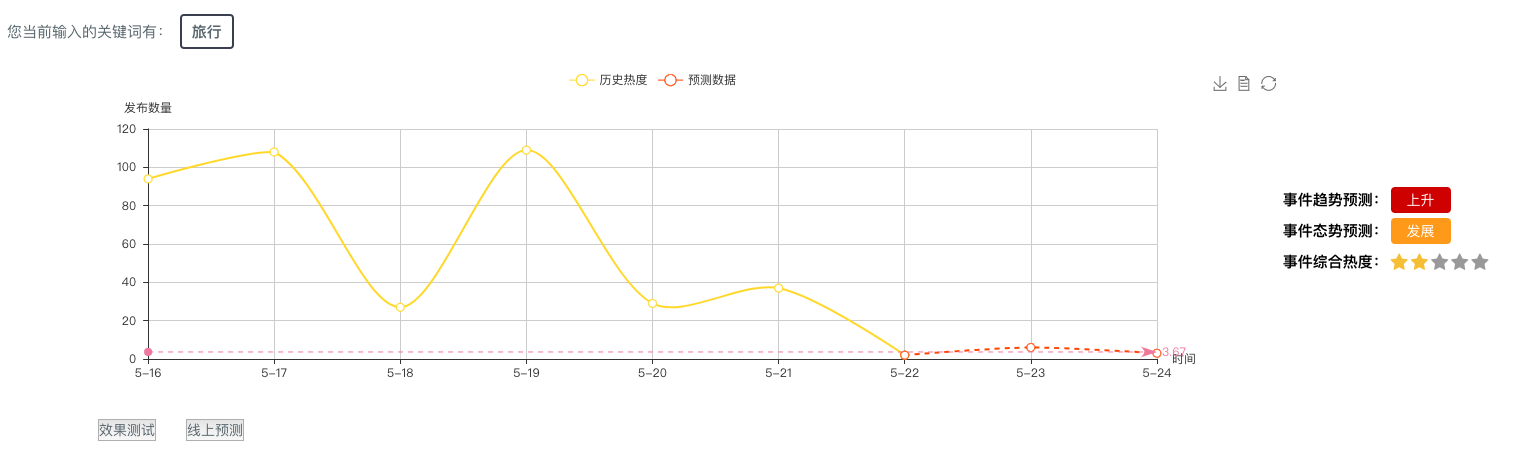
\includegraphics[width=1\textwidth]{fig_5_1_2_new}
    \bicaption{事件热度预测系统界面}{Public opinion data analysis system interface}
    \label{fig:figfivetwo}
\end{figure}

\section{系统架构}

事件热度预测系统架构如图\ref{fig:5_2}所示,本系统包含三个子系统,分别为业务 子系统,负责前端展示、任务提交、数据转发等功能,计算子系统负责核心算法 执行以及模型的更新,数据管理子系统负责和数据存储以及结果库的交互。

\begin{figure}[!htbp]
    \centering
    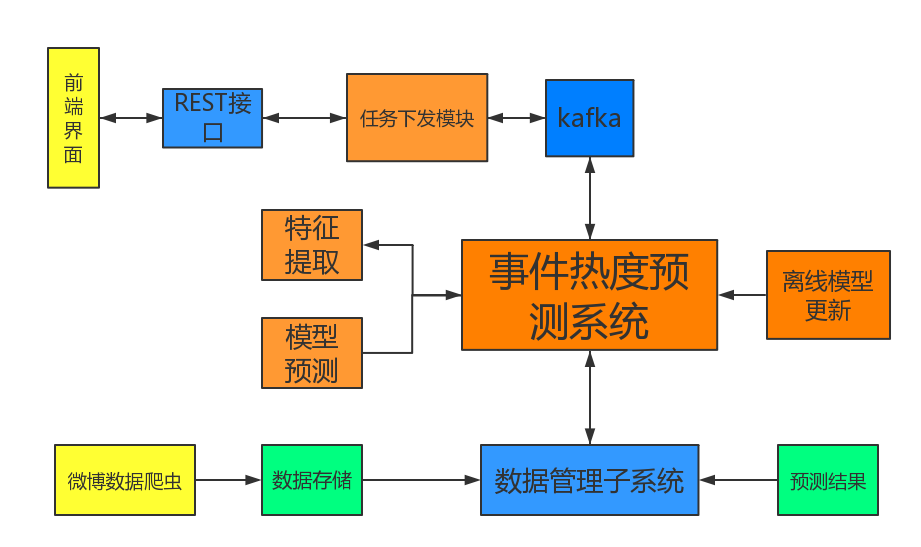
\includegraphics[width=1\textwidth]{5-2}
    \bicaption{系统模块架构图}{System module architecture diagram}
    \label{fig:5_2}
\end{figure}

事件热度预测系统层次架构图\ref{fig:5_3}如图所示,本系统从层次上可以分为四个 层次,从上层到底层可依次分为:展示层、业务层、计算层、存储层。其中展示 层负责数据结果的展示,业务层主要负责完成客户的业务逻辑功能,计算层负责 核心算法的执行,存储层负责业务数据以及结果数据的存储。

\begin{figure}[!htbp]
    \centering
    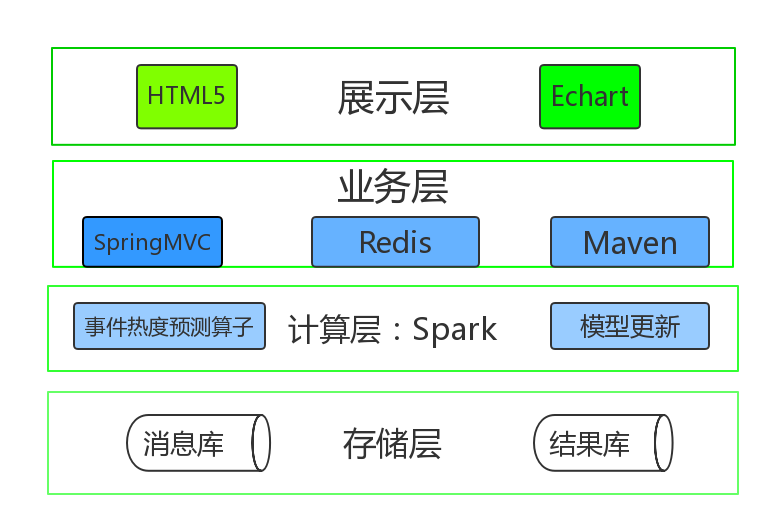
\includegraphics[width=1\textwidth]{5-3}
    \bicaption{系统层次架构图}{System hierarchy diagram}
    \label{fig:5_3}
\end{figure}

\section{微博数据模块}


微博数据模块每天都不断获取新的微博数据,然后进行基本解析,特征提 取,然后入库。微博数据字段如表 \ref{tab:t51} 所示。

\begin{table}[H]
    \centering
    \footnotesize% fontsize
        \bicaption{微博消息表}{Weibo Message Table}
      \label{tab:t51}
    \setlength{\tabcolsep}{30pt}% column separation
    \renewcommand{\arraystretch}{1.2}%row space 
    \begin{tabular}{cccc}
        \hline
         \textbf{序号} & \textbf{属性名称 }& \textbf{属性含义} &\textbf{ 数据类型}   \\
        %\cline{2-9}% partial hline from column i to column j
        \hline
         1 & $wb\_mid$ & 微博消息 ID & $string$ \\
         2 & $cont$ & 微博内容& $string$ \\
         3 & $uid$ & 用户 ID & $string$\\
         4 & $url$ & 微博链接 & $string$ \\
         5 & $nfri$ & 用户朋友数  &$int$ \\
         6 & $nfans$ & 用户粉丝数 & $int$ \\
         7 & $nfwd$ & 转发数量 & $int$ \\
         8 & $nrply$ & 回复数量 & $int$ \\
         9 & $pt$ & 微博发布时间 & $int$ \\
         10 & $loc$ & 微博地域 & $string$ \\
         11 & $message\_type$ & 微博消息类型& $int$ \\
         12 & $wb\_r\_mid$ & 微博根节点 ID & $string$ \\
         13 & $wb\_r\_uid$ & 微博根节点用户 ID & $string$ \\
         14 & $wb\_kw$ & 微博关键词 & $string$ \\
        \hline
    \end{tabular}
 
\end{table}
由于特征较多,一次计算时间过长,本文在获取到微博数据后就进行基本解 析,将其关键词,情感性以及地域信息及时存储,这样需要的时候,可以节约特 征提取的时间开销,当进行事件热度预测的时候就可以及时找到有关数据的特 征,提高系统的性能。



\section{事件预测模块}
本文的事件热度预测模块是根据 Hashtag 的流行度预测模型进行应用的,主 要是将 Hashtag 作为一个事件或者话题进行预测,这样既方便表示具体事件,又 具有一定的用户主观认识。事件预测大致分为三个模块,首先是事件任务下发模 块,这个是根据用户需要,选择相应时间段的微博数据进行分析,根据数据提取 出来的 Hashtag 标签,用户选择相应的感兴趣的事件进行任务下发;其次是事件 预测结果展示模块,根据用户提供的事件以及选择的时间范围,系统自动提取该 时间范围内模型所需的特征,进行事件热度预测,这个过程主要是特征提取的时 间消耗,模型的预测过程是实时响应的,因此后续的优化也主要是集中在特征的 高效提取上;由于微博数据实时更新,对于同一个任务,不同时刻的结果也应该是不同的,因此本文将其进行了自动更新,可以让用户及时查看最新结果。

\subsection{事件任务下发模块}
当用户新建一个任务时,首先需要用户选择观察的时间窗又,因为全量的数 据是庞大的,用户需要选择他感兴趣的时间范围内发生的事件,这样既便于用户 查找结果,也节省了资源的消耗,提高计算速度,新建任务流程如图\ref{fig:5_4}所示。


\begin{figure}[!htbp]
    \centering
    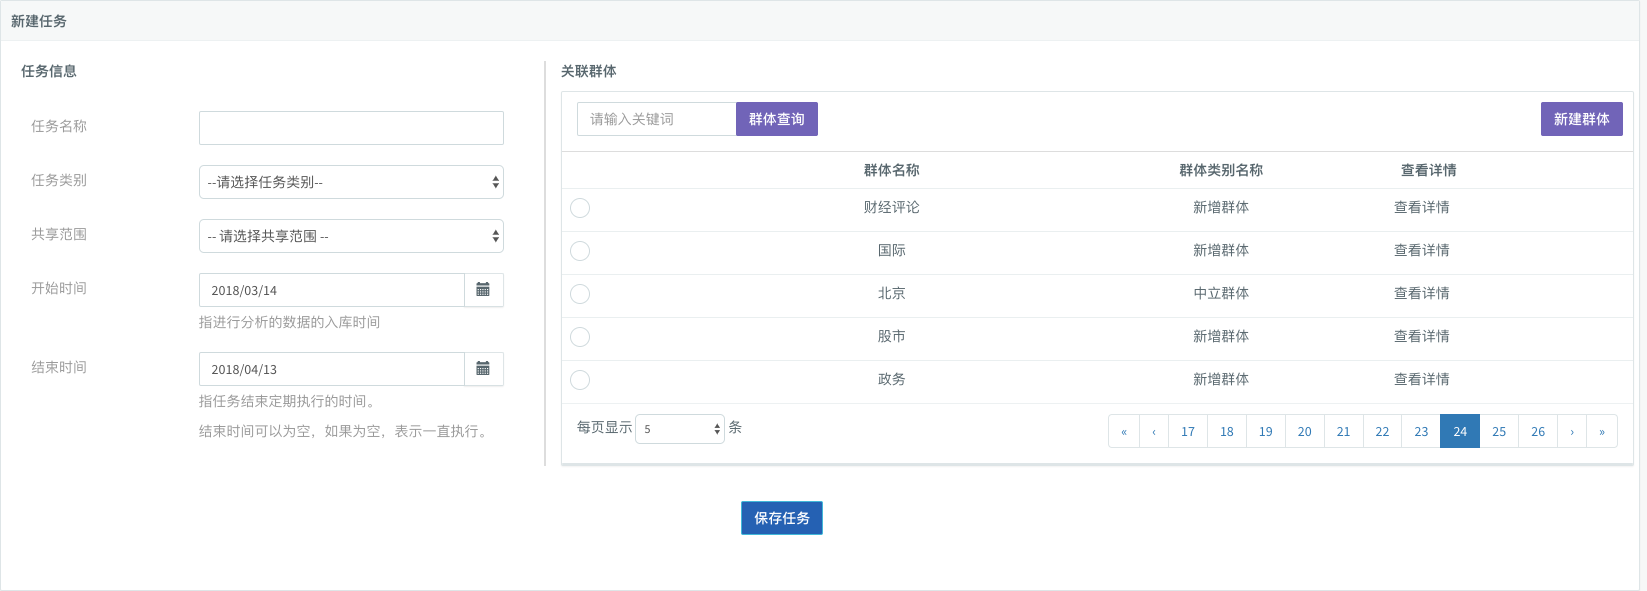
\includegraphics[width=1\textwidth]{hashtag_8}
    \bicaption{ 新建事件热度预测任务}{New Event Heat Prediction Task}
    \label{fig:5_4}
\end{figure}


任务下发以后,后台就根据用户选择的时间范围内的数据进行过滤,筛选, 提取特征,后台利用训练好的模型,对该时间段内的数据特征进行预测,任务等 待结果如图\ref{fig:5_5}所示。

\begin{figure}[!htbp]
    \centering
    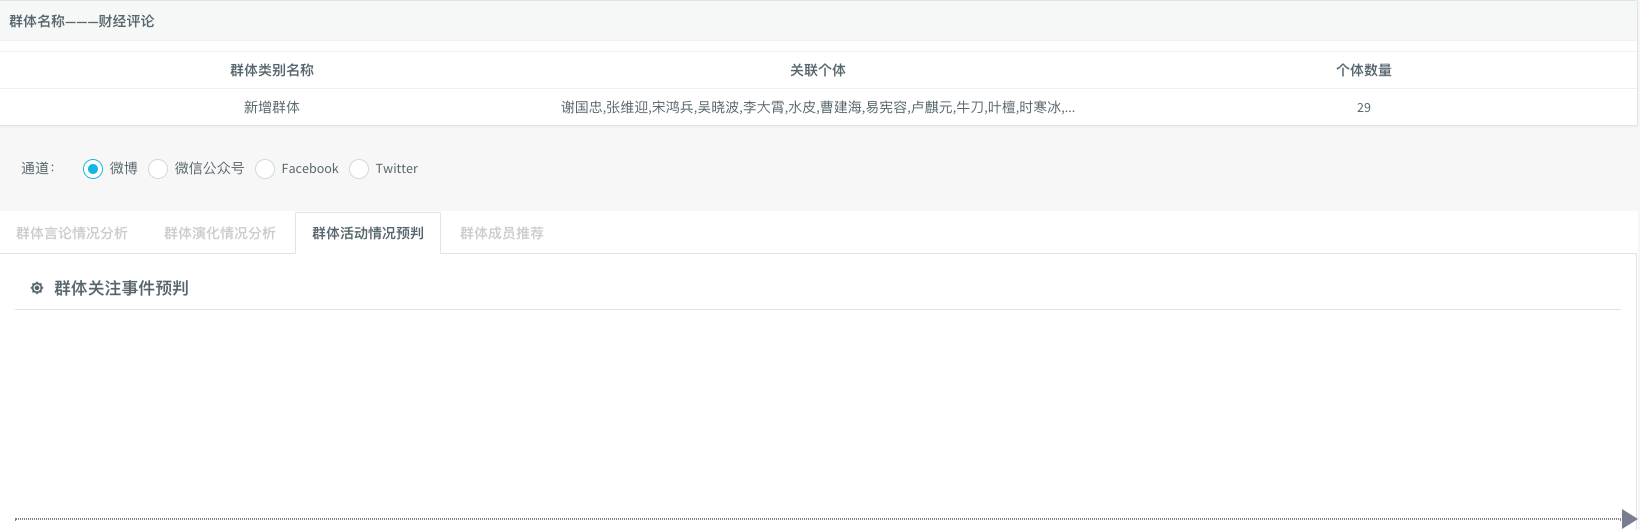
\includegraphics[width=1\textwidth]{hashtag_9}
    \bicaption{事件热度预测任务等待结果}{Event heat forecast task wait result}
    \label{fig:5_5}
\end{figure}

数据库中任务以及结果状态字段如表\ref{tab:t52} 所示,state 字段表示任务执行情况。

\begin{table}[H]
    \centering
    \footnotesize% fontsize
      \bicaption{事件热度预判任务表}{Event Heat Predictive Task Schedule}
      \label{tab:t52}
    \setlength{\tabcolsep}{30pt}% column separation
    \renewcommand{\arraystretch}{1.2}%row space 
    \begin{tabular}{cccc}
        \hline
         \textbf{序号} & \textbf{属性名称} & \textbf{属性含义 }& \textbf{数据类型 }  \\
        %\cline{2-9}% partial hline from column i to column j
        \hline
         1 & $id$ & 任务 ID & $int$ \\
         2 & $name$ &任务 ID& $string$ \\
         3 & $begin\_date$ & 任务开始时间 & $time$\\
         4 & $end\_date$ &任务结束时间 & $time$ \\
        	5 & $state$ & 任务状态& $int$\\
        	\hline
    \end{tabular}

\end{table}


\subsection{事件预测结果展示模块}

系统结果是通过 Kafka 实时反馈的,当系统将模型预测计算完成时,会将状 态位及时写入 Kafka,然后任务的状态位 state 就会显示计算成功, 这样就可以实 时获取计算结果,事件热度预判展示结果如图\ref{fig:5_6}所示。

\begin{figure}[H]
    \centering
    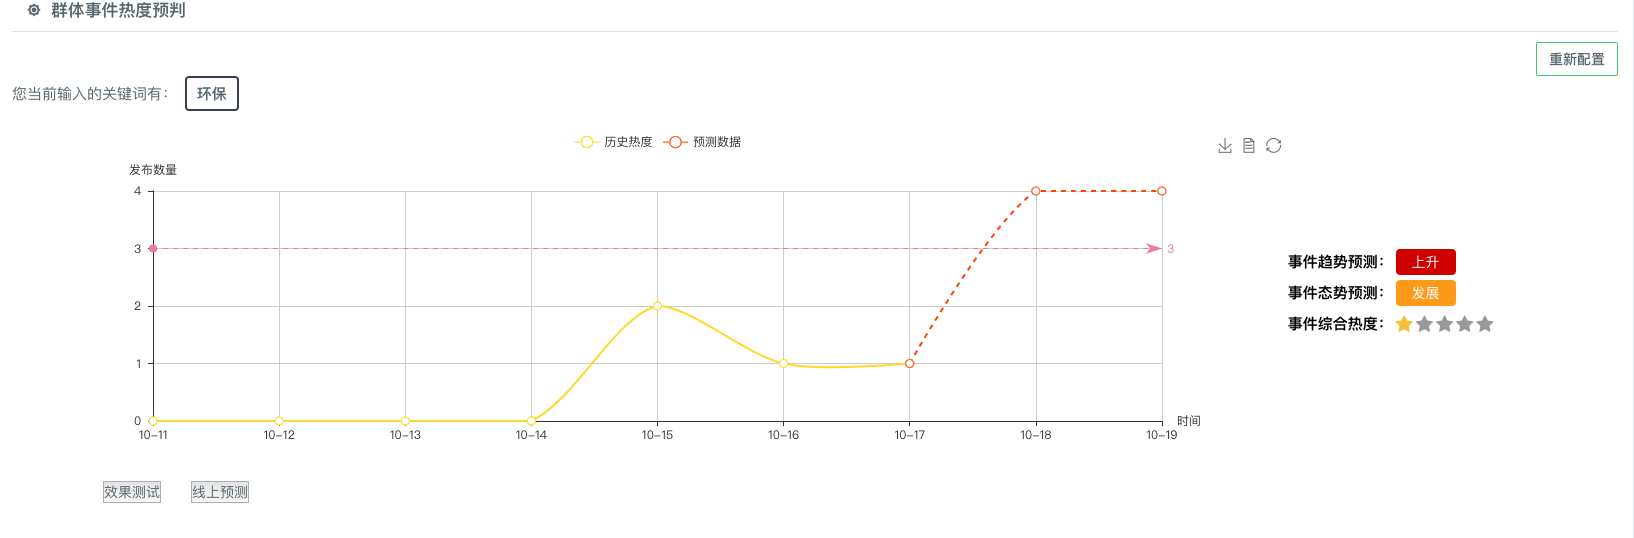
\includegraphics[width=1\textwidth]{hashtag_10}
    \bicaption{事件热度预判结果展示}{Event heat prediction results display}
    \label{fig:5_6}
\end{figure}

在该系统展示效果上,可以查看某一时刻的数据,让用户对该时间发生的事 件有更加清晰的认识,了解该事件的具体内容,数据展示如图\ref{fig:5_7}所示。

\begin{figure}[H]
    \centering
    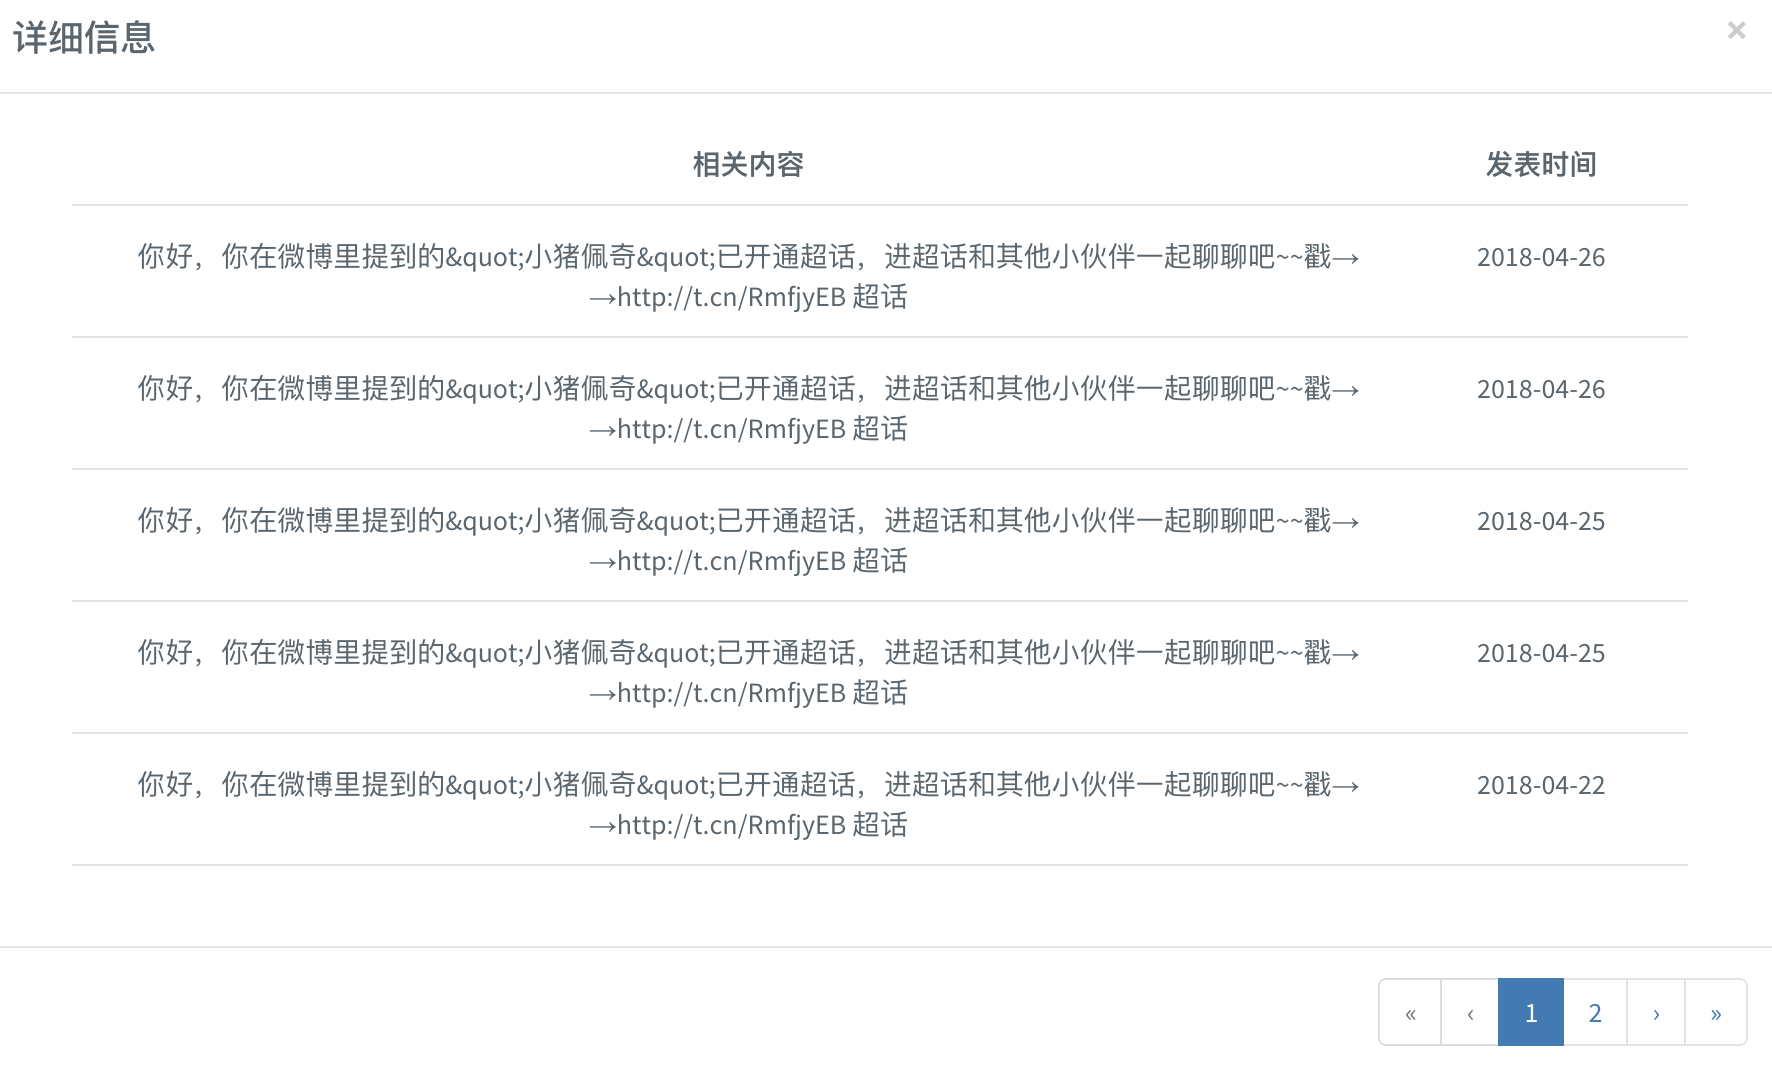
\includegraphics[width=1\textwidth]{hashtag_11}
    \bicaption{事件热度预判下的微博消息展示}{Event heat prediction microblogging message display}
    \label{fig:5_7}
\end{figure}


为了衡量系统的有效性,目前系统设计了线下结果与线上预测的对比,这样 既可以观察系统的有效性又可以给用户对于事件的一个直观长期的认识,效果 如图\ref{fig:5_11}所示,通过线下测试和线上预测的切换,可以查看其历史趋势, 通过之前 的预测结果与目前真实数据之间的对比,可以发现模型的预测结果整体上的趋 势是一致的,数据之间的准确性较高,验证了模型的有效性。


\begin{figure}[H]
    \centering
   
    \begin{subfigure}[b]{0.5\textwidth}
      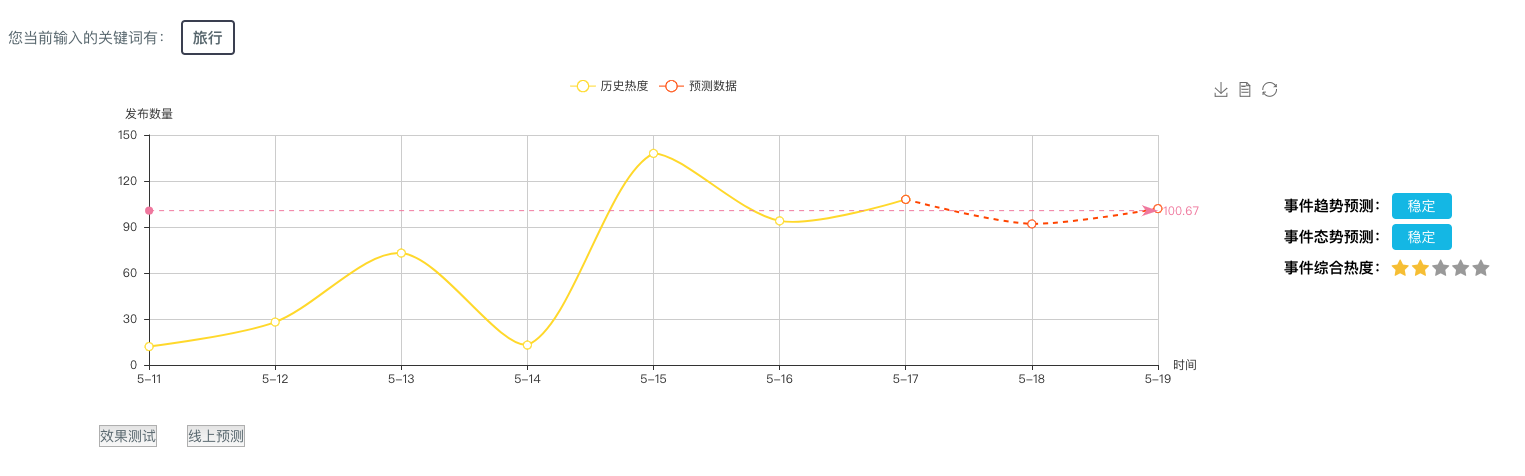
\includegraphics[width=\textwidth]{hashtag_17_new_1}
      \caption{}
      \label{fig:oaspl_a}
    \end{subfigure}%
    ~%add desired spacing
    \begin{subfigure}[b]{0.5\textwidth}
      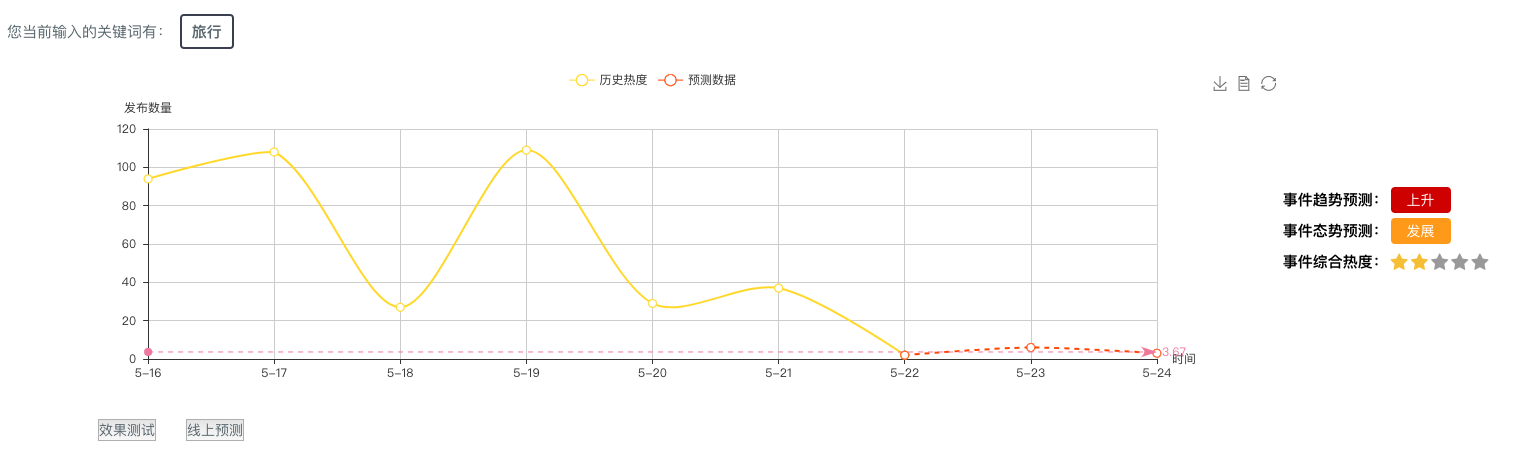
\includegraphics[width=\textwidth]{fig_5_1_2_new}
      \caption{}
      \label{fig:5_1}
    \end{subfigure}
    ~%add desired spacing
     \bicaption{事件预测结果对比。(a)线下预测,(b)线上预测}{Comparison of event prediction results.(a)Offline prediction,(b)Online prediction}
    \label{fig:5_11}
\end{figure}

\subsection{事件自动更新模块}
在本系统中,当用户执行了一个事件热度预测任务以后,由于他可能对此事 件持续关注,希望在长时间内对其了解,便于分析其长期趋势。一般的系统当一 个任务运算完成以后,该任务就处于结束状态,但是在本系统中考虑到数据的实
 时更新,以及用户对于任务的长期关注,本系统设定了任务的自动更新模块,当 用户希望长期关注某一事件以后,可以通过将任务的结束时间设置到未来某一 时刻,这样系统在每天凌晨都会根据结束时间与当前的比对来判断是否更新此 任务,从而实现了该任务的实时更新,确保了用户可以对此事件的长期关注,以 及及时获取最新结果数据。

\section{模型离线训练模块}
由于微博数据的实时性很强,为了能够及时响应最新数据,系统采用线下更
新模型和用户特征数据,这样可以保持一个实时最优模型。

\subsection{微博用户粉丝数据}
系统中包括用户粉丝网络结构的数据,数据结构如表\ref{tab:t53}所示,但是由于用 户关注的群体以及粉丝结构的不断变化,用户粉丝网络结构的向量表示应该实 时更新,但是那样对于系统的资源消耗过大,并且用户的粉丝并不是实时更新 的,短时间内用户粉丝网络结构更新的幅度很小,对于用户向量表示影响很小。 因此系统设计网络结构变化阈值,当用户粉丝结构数量变化达到总体的 10\%,系 统启动用户网络更新模型。

\begin{table}[H]
    \centering
    \footnotesize% fontsize
    \bicaption{微博用户关系表}{Weibo User Relationship Table}
      \label{tab:t53}
    \setlength{\tabcolsep}{30pt}% column separation
    \renewcommand{\arraystretch}{1.2}%row space 
    \begin{tabular}{cccc}
        \hline
         \textbf{序号} & \textbf{属性名称} & \textbf{属性含义} & \textbf{数据类型}   \\
        %\cline{2-9}% partial hline from column i to column j
        \hline
         1 & $fuid$ & 关注用户 ID & $string$ \\
         2 & $luid$ & 粉丝 ID& $string$ \\
         3 & $rlts$ & 用户粉丝之间关系 & $int$\\
         4 & $pt$ &  数据更新时间 & $int$ \\
        \hline
    \end{tabular}
     
\end{table}

\subsection{微博用户向量以及事件预测模型更新}
系统每天会采集大量的微博消息,Hashtag 以及微博消息的特性会随时变化, 它们已有的特征结构可能并不适合未来的事件预测,因此能够及时更新用户特 征,事件特征以及模型,对于预测结果的好坏是十分重要的,因此系统设计每周 末选取一定的数据量,进行用户粉丝网络结构的更新以及 Hashtag 模型的重新训 练,来保证模型的准确性。


\section{系统特色}
本系统具有如下特色:
\begin{enumerate}
\item  \bfseries 实时性 \mdseries 微博数据的采集过程是实时的,并且事件热度预测过程也是实时 更新的,所以整个系统的实时性能够得到保证。
\item  \bfseries 客户端友好 \mdseries 用户在新建任务时候,只需要填写关注时段和关注内容即可, 一键操作,系统可以实现实时更新,便于用户对于任务的查看和管理,并且即使 任务下发以后,用户关注的内容发生变化时,也不需要重新下发任务,只需要更 改关注字段即可,极大的方便用户的使用。
\begin{figure}[H]
    \centering
    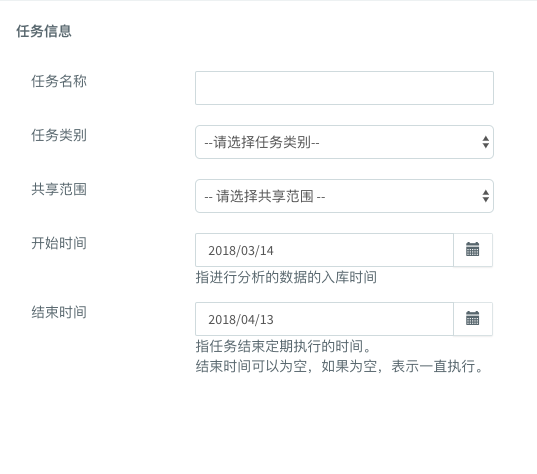
\includegraphics[width=1\textwidth]{hashtag_15}
    \bicaption{微博事件预测任务下发快捷方式}{Weibo event forecast tasks delivered shortcuts}
    \label{fig:5_10}
\end{figure}

\begin{figure}[H]
    \centering
    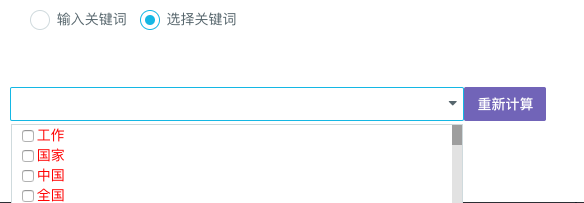
\includegraphics[width=1\textwidth]{hashtag_14}
    \bicaption{微博事件预测更改内容}{Weibo event prediction changes}
    \label{fig:5_9}
\end{figure}

\end{enumerate}

\section{本章总结}

在本文的前两章中,分别介绍了 Hashtag 流行度预测的两种方式,一种基于 特征的宏观预测,一种基于传播过程的多源微观预测。本章在介绍了微博数据采 集的相关情况后,通过将 Hashtag 作为微博的关注事件来进行预测,设计了一个 事件热度预测系统来进行事件热度预测。因为考虑时间效率以及模型的及时更 新,本系统采用基于特征的 Hashtag 流行度预测方式来进行设计,这样便于对结 果的分析。系统能够对采集到的数据以及用户下发的任务进行监控,并且系统可 以及时反馈预测结果,给用户提供了高质量的体验。系统通过对微博事件热度的 预测,能够辅助用户提前得知某一事件的未来趋势,对于评估网民的关注点有一 定的参考,具有较高的应用价值。